\documentclass[11pt,english]{article}
\usepackage{babel}
\usepackage[margin=1.3in]{geometry}
\usepackage{graphicx}
\usepackage{amsmath, amsfonts, amsthm, amssymb}
\usepackage{enumerate}
\usepackage{pdfpages}
\usepackage[toc,page]{appendix}
\usepackage{multicol}
\usepackage{enumitem}

%%%%%%%%%%%%%%%%%%%%%%%%HEADER%%%%%%%%%%%%%%%%%%%%%%%%%%%%%
\title{
{\normalsize \bf Technical Communication for Computer Scientists\\
Summer 2013}\\
\vspace{4cm}
{\bf Final Report:\\The Movie-Chain-Runner Project}}
\author{
\\Team Chain-Runner \\\\
Sung Uk Ryu\\
Eugene Scanlon\\
Shashank Singh\\
Jimmy Zong
}
%%%%%%%%%%%%%%%%%%%%%%%%%%%%%%%%%%%%%%%%%%%%%%%%%%%%%%%%%%%

\begin{document}

\pagenumbering{gobble} % exclude page-numbering for title page
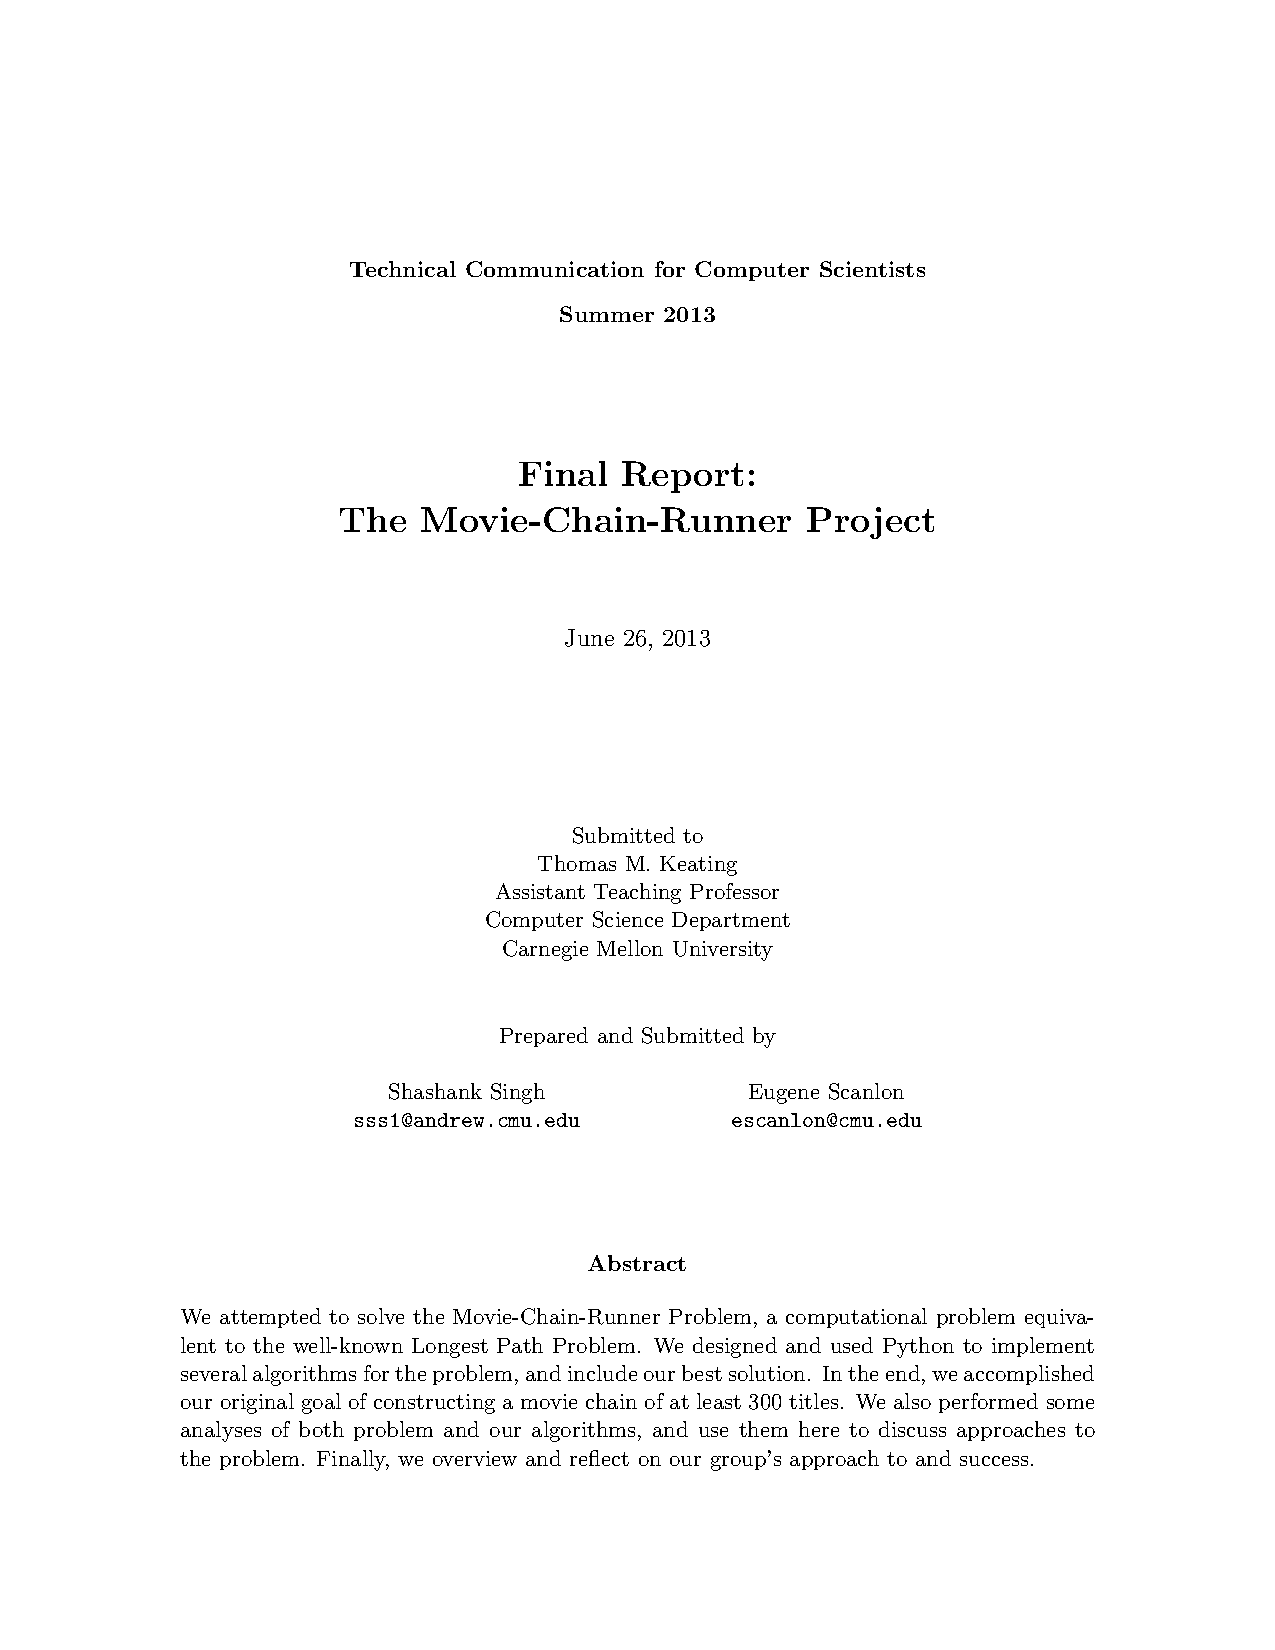
\includepdf{cover/cover.pdf}

\pagenumbering{roman} % include Roman page-numbering on ToC
\tableofcontents

\newpage
\pagenumbering{arabic} % include Arabic page-numbering starting here
\section{Introduction}
We first introduce the problem at hand and overview our solution and its
success.

\subsection{The Movie-Chain-Runner Problem}
The Movie-Chain-Runner Problem is to find the longest chain of overlapping
titles in a list of movie titles, where two titles are said to overlap if some
suffix of the first movie is identical to some prefix of the second movie. For
example, in the list
\begin{itemize}[noitemsep]
\item Day of the Dead
\item Live and Let Die
\item Dead Poets' Society
\item Die Another Day
\item The Last Samurai
\end{itemize}
the longest chain consists of 4 titles:

\begin{center}
Live and Let Die Another Day of the Dead Poets' Society
\end{center}

By appropriately representing the movie list as a graph, the Movie-Chain-Runner
Problem can be shown to be equivalent to the Longest Path Problem (finding the
longest simple path in a directed graph). The Longest Path Problem is well
known to be NP-Complete, meaning that no efficient algorithm exists to find
longest paths in large graphs, including our movie title graph. A review of the
literature reveals that good approximate longest paths also cannot be found
efficiently in large graphs.\hspace{-0.2cm}
\footnote{
A. Bj\"{o}rklund, T. Husfeldt, S. Khanna, ``Approximating longest directed
paths and cycles,'' Proc. of the 31st ICALP, 2004. (accessed June 26, 2013 at
\texttt{
http://citeseerx.ist.psu.edu/viewdoc/similar?doi=10.1.1.105.262\&type=ab}).}
Thus, our project is to study the movie title
graph and innovate ways to find long paths in the graph.

\subsection{Solution}
We constructed our 301 title chain in four major steps. Our first step to was to
reconstruct the list of movie titles as a directed graph, reducing the problem
to the well-known Longest Path Problem. The second step was to implement a
simple brute-force algorithm. The final two steps involved augmenting this
brute-force algorithm with two new procedures: ``reversal'' and ``insertion.''
The algorithms are described in detail on page 2, under the Algorithms
subsection of our Approach section.

\subsection{Did We Succeed?}
Our original goal was to surpass 300 titles. Despite some setbacks leading us
to lower our goal to 285 titles, we reached our original goal of 300 titles
with 301 titles (see Appendix B for the full movie chain). We did not
achieve our secondary goal of 328 titles needed to set a new record.

\section{Approach}

\subsection{Objectives}
We wanted our project's initial goal was to create a movie title chain of at
least 300 titles. Due to some early setbacks, we lowered this goal to 285
titles in our Progress Report, and kept 300 titles as an optional seconday
goal.

\subsection{Programming Languages}
Our team considered programming our Python, C, or MATLAB. We
settled on Python because our entire team was familiar with Python, whereas
only three team members had used C, and only two had used MATLAB. Although C
and MATLAB are faster languages, they are harder to use, and it would have
taken too much time for team members to learn either. Jimmy also wrote Bash
scripts to run our algorithms in parallel on cluster computers.

\subsection{Algorithms}
We present several algorithms (both successful and unsuccessful) we
considered.\\\\
\underline{Algorithms that worked:}

Our first attempt at a solution was a brute-force algorithm which greedily
followed every path in a depth-first search pattern, and retained the longest
path found. We ran this algorithm until it ceased to make appreciable progress
at a chain of 243 titles.

Our next step, ``reversal,'' was to reverse all edges in the movie graph and
use the brute force algorithm to extend the beginning of the 243 title chain.
We felt this approach would be useful because, upon running our original
algorithm multiple times, we found that the beginning of the chain changed
significantly, but end of the chain was always the same, suggesting that
the end of the chain was already nearly optimal. Again, we ran the algorithm
until it ceased to make appreciable progress, this time with a chain of 277
titles.

Our final step, ``insertion,'' checked if there was a longer subchain between
two titles in our 277 title chain. Simply attempting to ``squeeze'' chains in
between titles in our chain only increased our chain length to 278. However,
when we allowed the insertion algorithm to replace entire subchains
(``replacement''), we were able to construct our longest chain of 301 titles
before the algorithm ceased to make much progress.\\\\
\underline{Algorithms that didn't work:}

We tried an algorithm that computes acyclic subgraphs of our graph and then
runs a polynomial time Longest Path algorithm known for acyclic graphs.
However, the number of cycles proved too large to generate all the subgraphs,
and so we abandoned this effort.

We also considered some more elaborate algorithms we found in the literature:
a color-coding algorithm proposed by Alon et al.\hspace{-0.2cm}
\footnote{Noga Alon, Raphael Yuster, Uri Zwick, Color-coding, Journal of the
ACM (JACM), v.42 n.4, p.844-856, July 1995. (accessed June 16, 2013 at
\texttt{http://dl.acm.org/citation.cfm?id=210337}).}
and the genetic algorithms studied by Portugal et al.\hspace{-0.2cm}
\footnote{
D. Portugal, C. H. Antunes, R. Rocha, ``A Study of Genetic Algorithms for
Approximating the Longest Path in Generic Graphs,'' Proc. of the IEEE SMC, pp.
2539-2544, 2010. (accessed June 16, 2013 at
\texttt{http://ieeexplore.ieee.org/xpl/articleDetails.jsp?arnumber=5641920\&
navigation=1}).}
However, due to the complexity of implementing these algorithms and the success
of our simpler algorithms, we opted not to try them.

\subsection{Schedule}
Figure \ref{fig:gantto} below shows the original Gantt chart presented in
our project proposal. Figure \ref{fig:ganttn} below shows the revised Gantt
chart we presented in our progress report. The only changes were that the 300
title goal originally set for June 25 was eliminated and the 285 title goal
originally set for June 17 was extended to June 25. In practice, the only
deviation from our original schedule was achieving our 285 title goal one day
late (June 18), but we caught up by reaching our 300 title goal the next day
(June 19).
\begin{figure}[h]
\begin{center}
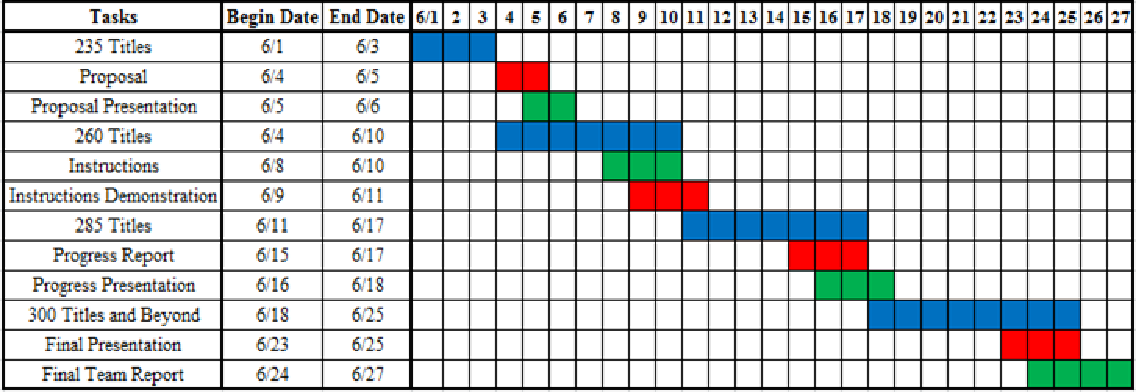
\includegraphics[width=\textwidth]{gantto}
\end{center}
\vspace{-7mm}
\caption{Our original Gantt chart.}
\label{fig:gantto}
\end{figure}
\begin{figure}[h]
\begin{center}
\includegraphics[width=\textwidth]{ganttn}
\end{center}
\vspace{-7mm}
\caption{Our revised Gantt chart.}
\label{fig:ganttn}
\includegraphics[width=0.2\textwidth]{key}
\end{figure}

\section{Discussion}
Here we present the project evaluation promised in our proposal, followed by
a discussion of lessons learned from the project and the resulting
recommendations for future groups.
\subsection{Evaluation}
As suggested in our proposal, we evaluated the success of our project using
three methods.\\\\
\underline{Method 1: Longest Chain Length}


{\bf Our project was a success} in that the number of titles in our longest
chain exceeded 300. Although we failed to establish a new record, this
secondary goal was optional and not expected.\\\\
\underline{Method 2: Algorithm Comparison}

Our second method of evaluation was to compare different algorithms to
decide on a ``best'' algorithm for the problem. Although we did not test a
diverse selection of algorithms, we did try several variants on the basic
brute force algorithm (as explained on page 2, under the the Algorithms
subsection of our Approach section. Table \ref{tab:algos} above presents the
longest chain found by each variant. It is clear from the results that both
reversal and replacement are important augmentations of the
basic brute-force algorithm.
\begin{table}
\centering
\begin{tabular}{l|c}
Algorithm                               & Longest Chain \\
\hline
Brute-Force                             & 243           \\
Brute-Force w/ reversal                 & 277           \\
Brute-Force w/ reversal and insertion   & 278           \\
Brute-Force w/ reversal and replacement & 301           \\
\end{tabular}
\caption{Longest chain found by each algorithm}
\vspace{-4mm}
\label{tab:algos}
\end{table}
\\\\
\underline{Method 3: Time Prediction}

In order to guage the difficulty of the problem at hand, we also attempted to
predict the time needed to solve the problem by exploring all possible paths
in the movie graph. To do this, we first measured the time taken to solve the
problem on many random subgraphs of the movie graph and used this data to fit
an exponential relation between the size of the graph and the time taken for
the computation. We then extrapolated this relation to conclude that performing
the computation on the entire graph would take about 1.03 trillion years,
approximately 100 times the lifespan of the sun. Appendix A gives a detailed
discussion of the experiment and its results and validity.

\subsection{Lessons Learned}
We learned several things about programming for large computational problems:
\begin{itemize}
\item Using primarily brute-force algorithms, we came quite close to (likely
within 13\% of) the optimal solution. Thus, although far from optimal in
theory, brute-force algorithms can produce decent solutions for some NP-hard
problems in practice.
\item For algorithms with large asymptotic runtimes, constant factors are
important - a 50\% runtime reduction is very significant when the algorithm can
take a day or more to run. This fact is really understated in CS classes.
\item With a high level language (like Python) it is crucial to consider all
available data structures and their implementations. We noticed too late that
using a set rather than a list for part of our code might have sped up our
program by a factor of 100.
\end{itemize}

\subsection{Recomendations}
Based on our experience, we strongly recommend attempting to implement simple
algorithms first when when tackling an NP-hard problem. While much of the
literature is focused on optimizing asymptotic performance, in practice, a well
implemented brute-force algorithm may perform nearly optimally with the time
and hardware available, while being much simpler to implement correctly.
Consequently, we also recommend trying to fully optimize code for such an
implementation fairly early, since much time can be wasted in running the
original program when one will later run a significantly optimized version.

Our team's work ethic and organization were crucial to our success. We
recommend having frequent meetings (at least twice weekly) in order to
coordinate work and ensure team members remain enganged.

\section{Sources}
\begin{itemize}
\item Gantt Chart created using software from the Gantt Project
(accessed June 4, 2013) 
\begin{itemize}
\item \texttt{http://www.ganttproject.biz/}
\end{itemize}
\item Git repository hosted on GitHub
(accessed June 4, 2013) 
\begin{itemize}
\item \texttt{https://github.com/}
\end{itemize}
\item Python Programming Language
(accessed June 4, 2013) 
\begin{itemize}
\item \texttt{http://www.python.org/}
\end{itemize}
\end{itemize}

\begin{appendices}

\section{Time Prediction}

\section{Our Longest Movie Chain}
Here, we include our current longest movie chain, with 278 titles and 885
words:
{\footnotesize
\begin{multicols}{2}
\begin{verbatim}
THE GOSPEL
THE GOSPEL OF JOHN
JOHN Q
Q AND A
A PERFECT MURDER
MURDER AND MURDER
MURDER IN THE FIRST
FIRST BLOOD
BLOOD DIAMOND
DIAMOND MEN
MEN WITH GUNS
GUNS OF THE MAGNIFICENT SEVEN
SEVEN YEARS IN TIBET
TIBET CRY OF THE SNOW LION
LION OF THE DESERT
DESERT BLUE
BLUE CAR
CAR 54 WHERE ARE YOU
YOU CANT TAKE IT WITH YOU
YOU LIGHT UP MY LIFE
LIFE WITH FATHER
FATHER OF THE BRIDE
BRIDE OF THE MONSTER
MONSTER HOUSE
HOUSE OF DRACULA
DRACULA DEAD AND LOVING IT
IT TAKES TWO
TWO OR THREE THINGS I KNOW ABOUT HER
HER MAJESTY MRS BROWN
BROWN SUGAR
SUGAR AND SPICE
SPICE WORLD
WORLD TRADE CENTER
CENTER STAGE
STAGE FRIGHT
FRIGHT NIGHT
NIGHT FALLS ON MANHATTAN
MANHATTAN MURDER MYSTERY
MYSTERY ALASKA
ALASKA SPIRIT OF THE WILD
THE WILD ONE
ONE NIGHT STAND
STAND IN
IN OLD CALIFORNIA
CALIFORNIA SPLIT
SPLIT SECOND
SECOND BEST
BEST OF THE BEST
THE BEST OF EVERYTHING
EVERYTHING RELATIVE
RELATIVE FEAR
FEAR STRIKES OUT
OUT OF THE PAST
PAST MIDNIGHT
MIDNIGHT RUN
RUN SILENT RUN DEEP
DEEP BLUE
DEEP BLUE SEA
SEA OF LOVE
LOVE HAPPY
HAPPY BIRTHDAY TO ME
ME MYSELF I
I SPY
SPY HARD
HARD TIMES
TIMES SQUARE
SQUARE DANCE
DANCE WITH A STRANGER
STRANGER IN THE HOUSE
THE HOUSE OF THE DEAD
DEAD BANG
BANG BANG YOURE DEAD
DEAD END
END OF DAYS
DAYS OF HEAVEN
HEAVEN CAN WAIT
WAIT UNTIL DARK
DARK CITY
CITY OF JOY
JOY RIDE
RIDE THE HIGH COUNTRY
COUNTRY LIFE
LIFE IS BEAUTIFUL
BEAUTIFUL GIRLS
GIRLS GIRLS GIRLS
GIRLS JUST WANT TO HAVE FUN
FUN AND FANCY FREE
FREE WILLY
FREE WILLY 2 THE ADVENTURE HOME
HOME ALONE
ALONE IN THE DARK
DARK STAR
STAR WARS EPISODE V THE EMPIRE STRIKES BACK
BACK TO THE BEACH
BEACH PARTY
PARTY GIRL
GIRL IN THE CADILLAC
CADILLAC MAN
MAN OF THE HOUSE
HOUSE OF FRANKENSTEIN
FRANKENSTEIN AND THE MONSTER FROM HELL
HELL NIGHT
NIGHT AND DAY
DAY FOR NIGHT
NIGHT AND THE CITY
CITY OF ANGELS
ANGELS WITH DIRTY FACES
FACES OF DEATH
DEATH SHIP
SHIP OF FOOLS
FOOLS RUSH IN
IN COLD BLOOD
BLOOD SIMPLE
SIMPLE MEN
MEN IN BLACK
BLACK AND WHITE
WHITE LIGHTNING
LIGHTNING IN A BOTTLE
BOTTLE ROCKET
ROCKET MAN
MAN ON FIRE
FIRE IN THE SKY
SKY HIGH
HIGH CRIMES
CRIMES OF PASSION
PASSION IN THE DESERT
DESERT HEARTS
HEARTS OF DARKNESS A FILMMAKERS APOCALYPSE
APOCALYPSE NOW
NOW YOU SEE HIM NOW YOU DONT
DONT BOTHER TO KNOCK
KNOCK OFF
OFF THE BLACK
THE BLACK ANGEL
ANGEL HEART
HEART CONDITION
CONDITION RED
RED DAWN
DAWN OF THE DEAD
DEAD HEAT
HEAT AND DUST
DUST TO GLORY
GLORY ROAD
ROAD HOUSE
HOUSE PARTY
PARTY MONSTER
MONSTER IN A BOX
BOX OF MOON LIGHT
LIGHT IT UP
UP CLOSE AND PERSONAL
PERSONAL BEST
BEST MEN
MEN DONT LEAVE
LEAVE HER TO HEAVEN
HEAVEN AND EARTH
EARTH GIRLS ARE EASY
EASY MONEY
MONEY FOR NOTHING
NOTHING BUT TROUBLE
TROUBLE IN PARADISE
PARADISE ROAD
ROAD GAMES
GAMES PEOPLE PLAY NEW YORK
NEW YORK NEW YORK
NEW YORK COP
COP LAND
LAND OF THE DEAD
DEAD MAN
DEAD MAN ON CAMPUS
CAMPUS MAN
MAN TROUBLE
TROUBLE EVERY DAY
DAY OF THE DEAD
DEAD OF NIGHT
NIGHT MOTHER
MOTHER JUGS AND SPEED
SPEED 2 CRUISE CONTROL
CONTROL ROOM
ROOM AT THE TOP
TOP GUN
GUN CRAZY
CRAZY AS HELL
HELL UP IN HARLEM
HARLEM RIVER DRIVE
DRIVE ME CRAZY
CRAZY PEOPLE
PEOPLE I KNOW
I KNOW WHAT YOU DID LAST SUMMER
SUMMER CATCH
CATCH A FIRE
FIRE ON THE MOUNTAIN
THE MOUNTAIN MEN
MEN CRY BULLETS
BULLETS OVER BROADWAY
BROADWAY DANNY ROSE
ROSE RED
RED EYE
EYE FOR AN EYE
AN EYE FOR AN EYE
EYE OF GOD
GOD TOLD ME TO
TO DIE FOR
FOR YOUR EYES ONLY
ONLY THE STRONG
ONLY THE STRONG SURVIVE A CELEBRATION OF SOUL
SOUL FOOD
FOOD OF LOVE
LOVE IS THE DEVIL
THE DEVIL RIDES OUT
OUT COLD
COLD FEVER
FEVER PITCH
PITCH BLACK
BLACK HAWK DOWN
DOWN WITH LOVE
LOVE LIFE
LIFE OR SOMETHING LIKE IT
IT HAPPENED AT THE WORLDS FAIR
FAIR GAME
GAME OF DEATH
DEATH WISH V THE FACE OF DEATH
DEATH WISH
WISH UPON A STAR
A STAR IS BORN
BORN AMERICAN
AMERICAN HISTORY X
X THE MAN WITH THE X RAY EYES
EYES OF AN ANGEL
ANGEL BABY
BABY SECRET OF THE LOST LEGEND
LEGEND OF THE LOST
THE LOST BOYS
BOYS AND GIRLS
GIRLS WILL BE GIRLS
GIRLS OF SUMMER
SUMMER LOVERS
LOVERS AND OTHER STRANGERS
STRANGERS WHEN WE MEET
MEET JOE BLACK
BLACK LIKE ME
ME WITHOUT YOU
YOU ONLY LIVE ONCE
ONCE AROUND
AROUND THE BEND
BEND OF THE RIVER
THE RIVER WILD
WILD THINGS
THINGS TO COME
COME AND GET IT
IT HAPPENED ONE NIGHT
ONE NIGHT WITH THE KING
THE KING AND I
I WANT TO LIVE
LIVE AND LET DIE
DIE MOMMIE DIE
DIE MONSTER DIE
DIE HARD
HARD EIGHT
EIGHT AND A HALF WOMEN
WOMEN IN LOVE
IN LOVE AND WAR
WAR OF THE WORLDS
THE WORLDS FASTEST INDIAN
INDIAN SUMMER
SUMMER SCHOOL
SCHOOL OF ROCK
ROCK STAR
STAR TREK THE MOTION PICTURE
PICTURE BRIDE
BRIDE OF THE WIND
THE WIND AND THE LION
THE LION KING
KING OF THE JUNGLE
JUNGLE 2 JUNGLE
JUNGLE BOOK
BOOK OF LOVE
LOVE WALKED IN
IN GODS HANDS
HANDS ON A HARD BODY
BODY DOUBLE
DOUBLE TEAM
TEAM AMERICA WORLD POLICE
POLICE ACADEMY
POLICE ACADEMY 3 BACK IN TRAINING
TRAINING DAY
DAY OF THE WOMAN
THE WOMAN IN RED
RED RIVER
RIVER OF NO RETURN
RETURN TO HORROR HIGH
HIGH SCHOOL HIGH
HIGH SPIRITS
SPIRITS OF THE DEAD
DEAD MAN WALKING
WALKING AND TALKING
TALKING ABOUT SEX
SEX AND THE OTHER MAN
MAN OF THE YEAR
YEAR OF THE DRAGON
DRAGON SEED
SEED OF CHUCKY
\end{verbatim}
\end{multicols}
}
\end{appendices}
\end{document}
